\documentclass{standalone}
\usepackage{pgfplots}
\pgfplotsset{compat=1.18}
\usepackage{siunitx}
\usepackage{tikz}

\begin{document}
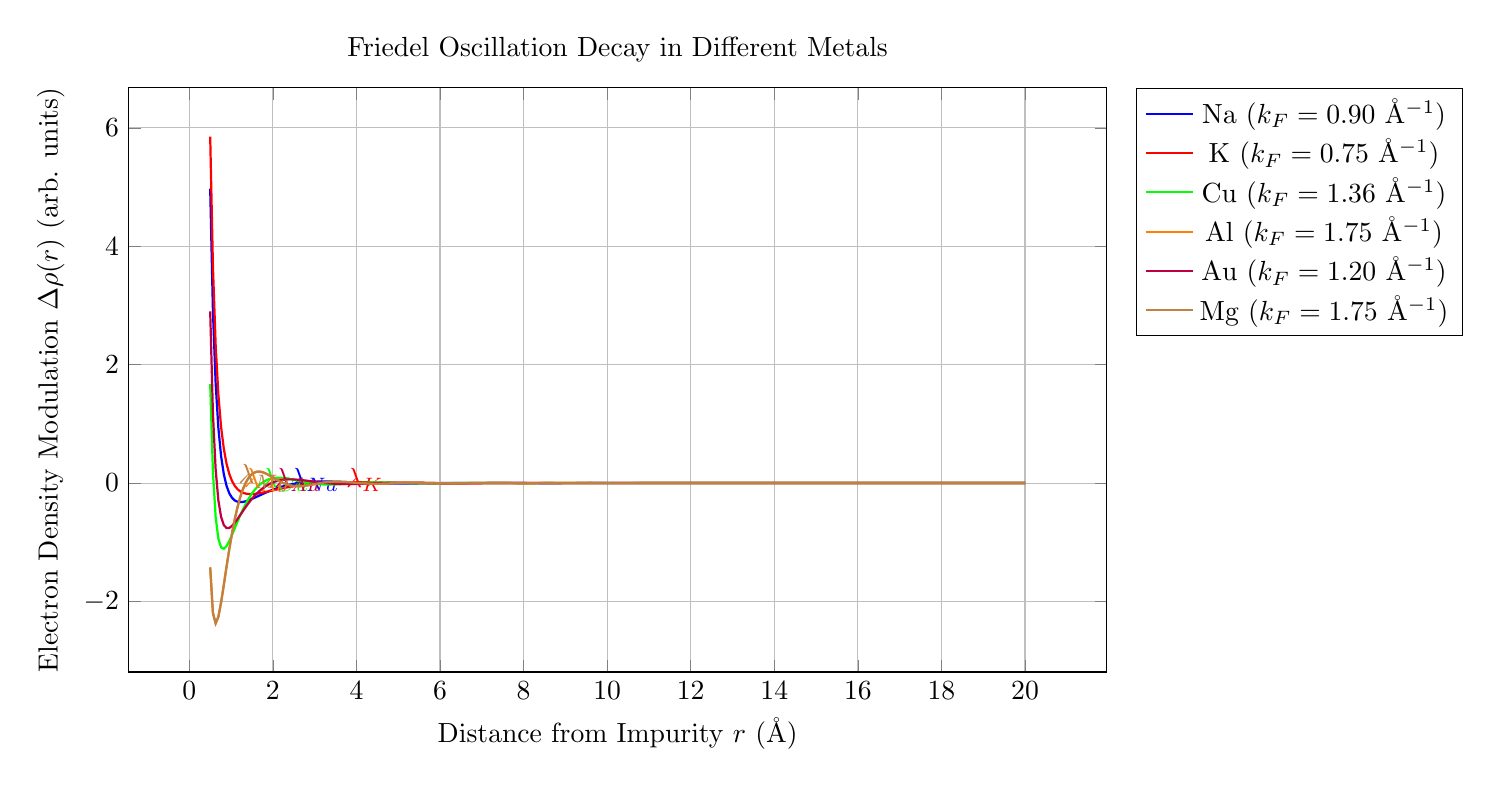
\begin{tikzpicture}
\begin{axis}[
    width=14cm,
    height=9cm,
    xlabel={Distance from Impurity $r$ (\AA)},
    ylabel={Electron Density Modulation $\Delta \rho(r)$ (arb. units)},
    legend pos=outer north east,
    grid=both,
    yminorgrids=true,
    xminorgrids=true,
    title={Friedel Oscillation Decay in Different Metals},
]

% Function for Friedel oscillation
\newcommand{\friedel}[2]{cos(deg(2*#1*x))/(x^3)}

% Sodium
\addplot[blue, thick, samples=300, domain=0.5:20] {\friedel{0.90}{x}};
\addlegendentry{Na ($k_F=0.90$ \AA$^{-1}$)}
\node[blue] at (axis cs:3,0.05) {$\lambda_{Na}$};

% Potassium
\addplot[red, thick, samples=300, domain=0.5:20] {\friedel{0.75}{x}};
\addlegendentry{K ($k_F=0.75$ \AA$^{-1}$)}
\node[red] at (axis cs:4.2,0.05) {$\lambda_{K}$};

% Copper
\addplot[green, thick, samples=300, domain=0.5:20] {\friedel{1.36}{x}};
\addlegendentry{Cu ($k_F=1.36$ \AA$^{-1}$)}
\node[green] at (axis cs:2.3,0.05) {$\lambda_{Cu}$};

% Aluminum
\addplot[orange, thick, samples=300, domain=0.5:20] {\friedel{1.75}{x}};
\addlegendentry{Al ($k_F=1.75$ \AA$^{-1}$)}
\node[orange] at (axis cs:1.8,0.05) {$\lambda_{Al}$};

% Potassium
\addplot[purple, thick, samples=300, domain=0.5:20] {\friedel{1.20}{x}};
\addlegendentry{Au ($k_F=1.20$ \AA$^{-1}$)}
\node[purple] at (axis cs:2.6,0.05) {$\lambda_{Au}$};

% Magnesium
\addplot[brown, thick, samples=300, domain=0.5:20] {\friedel{1.75}{x}};
\addlegendentry{Mg ($k_F=1.75$ \AA$^{-1}$)}
\node[brown] at (axis cs:1.8,0.08) {$\lambda_{Mg}$};

\end{axis}
\end{tikzpicture}
\end{document}
